\section{Shape index and query-shape containment}

We define a Shape Index (SI) as a set of mappings between RDF data shapes and sets of resources.
Additionally, an SI has an associated domain (set of URLs)
and a flag indicating if the SI is \emph{complete}.
A SI is complete when every resources in the domain is associated with a shape.
In a SI when a shape is in relation to a set of RDF resources then the shape must validate them.
Furthermore, every set of triples respecting the shape in the domain must be located inside one resource of the set.

Our approach consists of determining before the traversal of a whole domain the location of the useful resources for the query execution
resulting in the pruning of links leading to surely non-contributing resources.
For that purpose, the query engine must first discover the SI in each (sub)domain.
In the case of Solid, the SI should be at the root of the pod to be easily discoverable.
Source selection with an SI consists of interpreting the binding results from a \emph{query-shape containment} problem similar to the classic query containment problem.
We propose that we can transform a shape into a query ($Q_{s}$).
In this short paper, we don't provide proof for this proposition, however, 
\citeauthor{Delva2021} give an intuition by demonstrating how to query RDF subgraphs using RDF data shapes as a query language.
The algorithm divides the query into multiple star patterns with their dependencies ($Q_{star}$).
Then we evaluate if the  $Q_{star}$ are contained inside the $Q_s$ of the SI.
If all the $Q_{star}$ are contained in a $Q_{s}$ or have no binding with any $Q_{s}$
we adapt the reachability criteria to ignore all the resources not linked to a $Q_{s}$ even if the SI is \emph{incomplete}.
If the SI is \emph{complete} and not all the $Q_{star}$ are contained in a $Q_{s}$ the reachability criteria can be adapted
to visit every resource in relation to a $Q_{s}$ with a partial binding with a $Q_{star}$. 
In the case of an \emph{incomplete} SI the algorithm can only discover resources.

\begin{figure}[h]
    \centering
    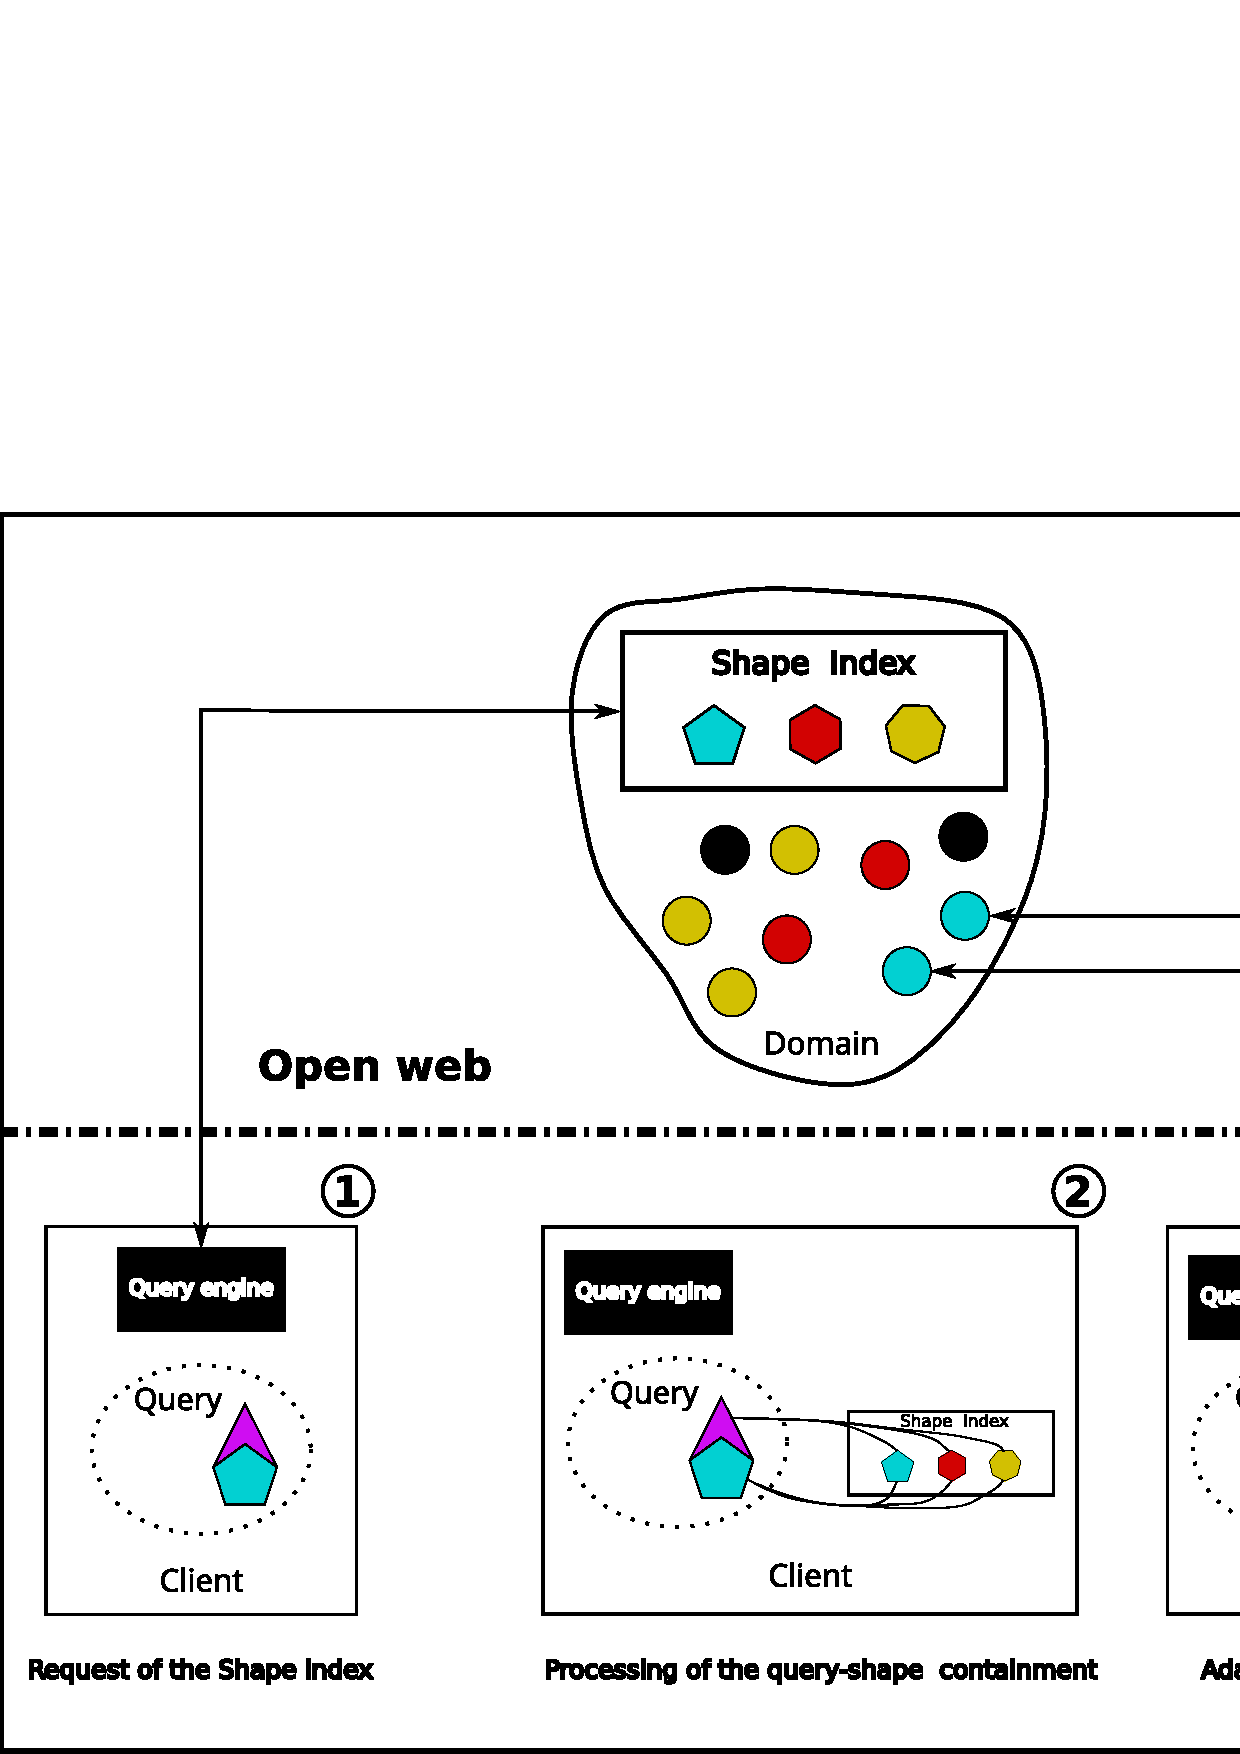
\includegraphics[width=0.45\textwidth]{figure/shape_containement_v2}
    \caption{A schema of the source selection when an engine encounters a SI. It first dereference it, 
    then it performs the \emph{query-shape containment} and lastly, it dereference only the resources that might contribute to the query execution.}
    \label{fig:shape_index}
\end{figure}